% Week 4: Convolutional Neural Networks I
\chapter{Convolutional Neural Networks I}
\label{ch:week4}

\section*{Computer Vision Tasks}

\begin{figure}[H]
    \centering
    \includegraphics[width=1\linewidth]{images/week_4/Screenshot 2024-10-22 at 17.49.34.png}
    \caption{Computer Vision}
    \label{fig:enter-label}
\end{figure}

\section*{Human vs Computer Image Analysis}

\textbf{Humans}
\begin{itemize}
    \item Look for local features
    \item Ignore irrelevant info
\end{itemize}

\textbf{Computer}
\begin{itemize}
    \item Matrix of pixels
    \item Light intensity of pixel: numerical value (typically between 0 - 255)
    \item Color channels
    \begin{itemize}
        \item Typically 3 channels (RGB)
        \item Can be hyperspectral (100s of channels)
    \end{itemize}
\end{itemize}

\section{Challenges Solved by Convolutional Layers}

\begin{tcolorbox}
    CNNs Motivation:
    \begin{enumerate}
        \item Reduce parameters.
        \item Leverage local connectivity.
        \item Deal with translation invariance \& equivalence (treats results same local result irrespective of where it is).
    \end{enumerate}
\end{tcolorbox}

\subsection{Context: Fully Connected Layers}

So far we only worked with “fully connected” layers, where every node is connected to every node of the next
layer.


\begin{figure}[H]
    \centering
    \includegraphics[width=0.5\linewidth]{images/week_4/fully connected.png}
    \caption{Fully Connected network}
    \label{fig:enter-label}
\end{figure}

Mathematically, we represent the activation of a neuron in the next layer as:

\[
h^{[l]}_j = \sigma \left( \sum_{i=1}^{H^{[l-1]}} W^{[l]}_{ij} h^{[l-1]}_i + b^{[l]}_j \right)
\]

\textcolor{red}{should this be $a$?}

Here:
\begin{itemize}
    \item $h^{[l-1]}_i$ represents the activations from the previous layer ($l-1$),
    \item $W^{[l]}_{ij}$ is the weight connecting neuron $i$ in layer $l-1$ to neuron $j$ in layer $l$,
    \begin{itemize}
        \item NB: summation over $i$: summing over weighted inputs from the prev layer into the next layer node
    \end{itemize}
    \item $b^{[l]}_j$ is the bias term for neuron $j$ in layer $l$,
    \item $\sigma(\cdot)$ is the activation function (often ReLU or sigmoid).
\end{itemize}

\subsection{Convolutional Layers: Images and input features}

For image analysis and other applications, another type of layer has been very successful: \textbf{convolutional layers}.

\subsubsection*{Challenge 1: Spatial structure and local connectivity}

\textit{\textbf{Problem}: Nearby pixels are often related!}\\

In fully connected layers, the spatial information present in input data like images is not preserved:
\begin{itemize}
    \item To feed an image into a fully connected network, the image must first be 'flattened': transformed into an array of pixels.
    \item The result is a vector where each pixel is taken as one feature.
    \item Every pixel is treated independently, which can lead to inefficiency when dealing with structured data like images. 
\end{itemize}

The result is that each pixel is a separate feature, and this representation discards important information about the spatial relationships (spatial correlations) between nearby pixels.\\

\begin{tcolorbox}
    \textit{\textbf{Solution:} Convolutional Layers and Local Connectivity}\\

    Convolutional layers preserve the spatial structure of the input. Instead of treating each pixel independently, convolutional layers apply filters (or kernels) across the image to detect patterns like edges, textures, or objects.\\
    
    In a convolution operation, we slide a small kernel over the input image. For example, given an image $X \in \mathbb{R}^{d_x \times d_y}$ and a kernel $K \in \mathbb{R}^{r \times r}$, the convolution is computed as:
    \[
    (X * K)_{i,j} = \sum_{p=0}^{r-1} \sum_{q=0}^{r-1} x_{i+p, j+q} k_{r-p, r-q}
    \]
    
    The kernel detects specific features at different locations in the image, such as edges, corners, or textures, regardless of their position. This helps achieve \textbf{translation invariance}, meaning the network can recognize patterns regardless of where they appear in the image.
\end{tcolorbox}

\subsubsection*{Challenge 2:  High-dimensional Image Inputs}

\textit{Problem: we want high performance \& less parameters!}\\

Images typically contain thousands or millions of pixels, leading to very high-dimensional input spaces. For example:
\[
\text{Image size} = 28 \times 28 = 784 \text{ pixels for a small grayscale image.}
\]

When we work with images, like a (small) $1$ MB image:
\[
\text{Image size} = 10^6 \text{ pixels.}
\]

If we were to fully connect such a large input image to a hidden layer with $1000 (10^3)$ units, the number of parameters we would need to train is:
\[
10^6 \times 10^3 = 10^9 \text{ parameters.}
\]

This huge number of parameters makes training challenging, requiring a lot of \textbf{computational power} and leading to possible \textbf{overfitting}. Additionally, this method does not exploit the spatial structure of images, where nearby pixels are often related.

\begin{tcolorbox}
    \textit{\textbf{Solution:} Convolutional layers share weights \& Pooling Layers reduce dimensionality}
\end{tcolorbox}

\subsubsection*{Challenge 3: Translation Invariance and Equivariance}

\textit{Problem: We need a new type of layer to work as such a \textbf{“detector”}}\\

In image processing tasks, when detecting objects, we care about the \textit{presence} of the object but not their exact position. Convolutional layers are designed to be translation invariant, meaning they focus on detecting patterns regardless of where they appear in the input.\\

\begin{tcolorbox}
    \textit{\textbf{Solution:} kernel filters}\\
    
    In a convolutional layer, the filter acts as a feature detector (e.g., helmet detector) that slides over the entire image to find areas that match. \\

    Furthermore, CNNs also exhibit \textbf{equivariance}, meaning that if the input shifts, the output also shifts by the same amount. This makes them especially useful for tasks like object detection.
\end{tcolorbox}

\textbf{Example: Cat Image Feature Detection}\\

Consider the task of classifying an image of a cat. Different filters can be used to detect different parts of the cat, such as its eyes or nose. For example, one filter might activate when it detects an eye, and another when it detects the nose. These activations help the network recognize that the image contains a cat, even if the cat's position in the image changes.\\

In this case, different parts of the image correspond to different filters, and the combination of these feature detectors enables the network to classify the image accurately.


\section{Properties of CNNs}

CNNs are widely used in Computer Vision. Also, competitive in exploiting one-dimensional sequence structure in time series analysis, audio and text. This is because of:\\

\textbf{Local Connectivity}\\

Convolutional neural networks (CNNs) contain convolutional layers that leverage dependencies of nearby features. \\

This property allows CNNs to exploit the spatial relationships within images more efficiently than fully connected networks.\\

\textbf{Translation Invariance and Equivariance}.\\

CNNs exhibit \textbf{translation invariance}, which means that the exact position of features within the image is less important. For example, whether an object like a cat is on the left or right of an image, a CNN can still detect it effectively. This is achieved through the sliding window mechanism of convolutional layers, where filters (or kernels) are applied across the image at every position.\\

CNNs also have \textbf{equivariance}, meaning that a shift in the input results in a corresponding shift in the output. If the features in the input image shift by some pixels, the output of the convolutional layer will shift accordingly, preserving the structure of the features.\\

\textbf{Locality} \\

CNNs focus on \textbf{locality} in early layers by analyzing small regions of the input image (local features like edges, corners). As you move deeper into the network, the layers begin to combine local features into more global, high-level features (such as objects). This hierarchical approach allows CNNs to detect complex structures in images by combining simpler ones.\\

\textbf{Invariance to Illumination}: \\

CNNs can also handle variations in illumination. Because they focus on extracting patterns and shapes from the image, changes in brightness do not drastically affect their performance. The filters in CNNs adapt to detect features like edges, which remain consistent even under different lighting conditions.\\

\textbf{Computational Efficiency}

\begin{itemize}
    \item CNNs require \textbf{fewer parameters} compared to fully connected networks. This is because filters are \textbf{shared} across the image, meaning that the same weights are applied to different regions of the image. This weight sharing reduces the total number of parameters and makes CNNs easier to train.
    \item CNNs are highly \textbf{parallelizable}. The convolution operation can be performed simultaneously across multiple parts of the image, making CNNs well-suited for \textbf{GPU} acceleration, significantly speeding up training.
\end{itemize}

\subsection{Versatility}

CNNs are not only limited to computer vision tasks. They are also highly effective in \textbf{one-dimensional sequence analysis}, such as:
\begin{itemize}
    \item \textbf{Time series analysis}, where the temporal relationships in the data can be captured by treating the sequence similarly to how images are processed.
    \item \textbf{Audio processing}, where sound wave patterns can be analyzed using CNNs in a manner similar to how images are processed.
    \item \textbf{Text analysis}, especially for tasks like sentiment analysis or language modeling, where convolutional layers help detect important sequences of words or characters.
\end{itemize}

\section{Discrete Convolution Operations}

The purpose of the convolution is to apply a small filter or \textbf{kernel} across an image (or any input data) to extract meaningful features.\\

This is a grid / matrix of learned features.

\subsection{Definition of Discrete Convolution}

Consider an image input $X \in \mathbb{R}^{d_x \times d_y}$, which is a matrix of pixel values, and a kernel $K \in \mathbb{R}^{r \times r}$, which is a smaller matrix representing a filter. The discrete convolution is computed as:

\[
(X * K)_{ij} = \sum_{p=0}^{r-1} \sum_{q=0}^{r-1} x_{i+p, j+q} k_{r-p, r-q}
\]

In this operation:
\begin{itemize}
    \item $X$ is the input image (or matrix),
    \item $K$ is the kernel (or filter), and
    \item $(i, j)$ are the indices for the top-left corner of the region in $X$ where the filter is currently being applied.
\end{itemize}

The offsets $p$ (rows) and $q$ (columns) run from $0$ to $r-1$, where $r$ is the size of the kernel. Each element of the kernel is multiplied with the corresponding element of the image at the current location, and the results are summed to give the output value at $(i, j)$.

\subsection{Example of Discrete Convolution}

Let's compute the convolution for the following example, where the kernel size is $r = 2$ and the input matrix $X$ and kernel $K$ are given as:

\[
X = 
\begin{bmatrix}
0 & 80 & 40 \\
20 & 40 & 0 \\
0 & 0 & 40
\end{bmatrix}, \quad
K = 
\begin{bmatrix}
0 & 0.25 \\
0.5 & 1
\end{bmatrix}
\]

We use the discrete convolution formula:
\[
(X * K)_{ij} = \sum_{p=0}^{r-1} \sum_{q=0}^{r-1} x_{i+p, j+q} k_{r-p, r-q}
\]
where $r = 2$, and the offsets $p$ and $q$ run from $0$ to $1$. \\

Notice the minus sign in the indices of $k$: We can think of this as a filter $\tilde{K}$, which is the kernel $K$ with \textbf{rows and columns flipped}. This simplifies the operation considerably.\\

The flipped kernel $\tilde{K}$ is:

\[
\tilde{K} = 
\begin{bmatrix}
1 & 0.5 \\
0.25 & 0
\end{bmatrix}
\]

Now, applying the convolution at position $(i,j)$ on the top-left corner of the image matrix $X$, we compute:

\[
1 \cdot 0 + 0.5 \cdot 80 + 0.25 \cdot 20 + 0 \cdot 40 = 45
\]

Thus, the output value at $(i,j)$ is $45$.

\subsection{Purpose}

This discrete convolution operation allows the network to detect local patterns (such as edges, textures, etc.) by applying small kernels across the input. \\

This process is repeated for each position in the image, with the result being a feature map that highlights the areas where the filter detects relevant patterns.

\section{Discrete Cross Correlation Operation}

\begin{tcolorbox}
    The term \textbf{Convolutional Neural Network (CNN)} originates from the mathematical concept of convolutions.\\

    However, what is actually computed in most CNN implementations is \textbf{cross-correlation}, not convolution in the strict mathematical sense. \\
    
    While convolution requires flipping the kernel before applying it to the input, cross-correlation does not. Despite this difference, the operation is functionally equivalent for the purpose of feature extraction in neural networks, as both capture local dependencies and patterns in the data efficiently.

\end{tcolorbox}

\subsection{Using Convolutional Kernels as Weights}

In convolutional layers, the filters or \textbf{kernels} act as weight matrices for the input data. The role of the kernel is to extract important features from the input, such as edges or textures in an image. \\

Here's an important consideration regarding how these kernels function as weights:

\subsubsection*{Order of Weights}

For the computer, the order in which the weights are applied does not matter as long as it is consistent throughout the convolution operation. This means that the order of the rows and columns of the kernel can be flipped, and the operation will still yield the same result. This concept leads us to define a flipped kernel $\tilde{K}$ as our \textbf{weight matrix}:
\[
\tilde{K} = W
\]
where $W$ is the set of learnable weights for the layer. Flipping the rows and columns of the kernel simplifies some convolution operations, but it doesn't change the core concept of applying a filter to an image.

\subsubsection*{Cross-correlation vs Convolution}

While the operation in convolutional layers is referred to as "convolution", it is technically a form of \textbf{discrete cross-correlation} between the input $X$ and the weight matrix $W$. \\

Mathematically, cross-correlation between an input $X$ and kernel $W$ is written as:
\[
(X * W)_{ij} = \sum_{p=0}^{r-1} \sum_{q=0}^{r-1} x_{i+p, j+q} w_{p,q}
\]
where the kernel is not flipped as it would be in the mathematical definition of convolution.

\subsubsection*{Activation of Hidden Layers}

The output of the convolution or cross-correlation operation forms the activation of our hidden convolutional layer. The result of this operation is an \textbf{activation map} that highlights the regions of the input that correspond to the learned features of the kernel.

\subsubsection*{Non-linear Activation Function}

After applying the convolution, we introduce non-linearity into the model by applying a \textbf{non-linear activation function} to the resulting activation matrix. For instance, we can apply a sigmoid function to each entry of the activation matrix. \\

This non-linearity allows the network to model more complex patterns in the data by stacking multiple convolutional layers with activations.

\section{Effect of Applying a Convolution}



We apply a \textbf{convolution} to the input matrix $X$ using a kernel $K$. The convolution operation slides the kernel across the input, performing \textbf{element-wise multiplication} and \textbf{summing} the results to produce an output matrix $X * K$.\\

\textit{NB: In this example, the kernel is the same as the kernel/weights with the rows and columns flipped}\\

\textbf{Pixel matrix:}
\[
X = \begin{bmatrix}
0 & 0 & 255 & 0 & 0 \\
0 & 0 & 255 & 0 & 0 \\
0 & 0 & 255 & 0 & 0 \\
0 & 255 & 0 & 0 & 0 \\
255 & 0 & 0 & 0 & 0 \\
\end{bmatrix}
\]

\textbf{Kernel matrix:} the convolution highlights the areas that are similar to the filter.
\[
K = \begin{bmatrix}
0 & 0.5 \\
0.5 & 0
\end{bmatrix}
\]

\textbf{Resulting matrix $X * K$:} contains values that represent the presence of features detected by the kernel. 
\[
X * K = \begin{bmatrix}
0 & 128 & 128 & 0 \\
0 & 128 & 128 & 0 \\
0 & 255 & 0 & 0 \\
255 & 0 & 0 & 0
\end{bmatrix}
\]

\subsection{Feature Detection}

The convolution highlights areas of the input image \textbf{that are similar to the pattern represented by the kernel}. For instance, the kernel in this example is detecting changes in intensity along edges, and the output matrix highlights these areas with higher values (e.g., 128 or 255).

\subsection{Non-linear Activation}

Once the convolution is performed, the result can be passed through a non-linear activation function.\\

By applying this activation function to each entry of the resulting matrix, we can obtain an output where neurons corresponding to strong feature activations (such as edges) are highlighted.\\

This process allows the network to focus on relevant areas of the image, and successive layers can further refine these features, eventually leading to high-level feature detection.

\subsection{Example: Change from dark to light}

\begin{figure}[H]
    \centering
    \includegraphics[width=1\linewidth]{images/week_4/convolution.png}
    \caption{NB: this is a correlation operation}
    \label{fig:enter-label}
\end{figure}

\section{Padding}

\subsection*{Loosing Information at the Edges of the Input}

When applying a convolutional filter to an image, we encounter a common issue at the edges of the input: the filter may not have enough neighboring pixels to perform a full convolution, which can result in losing information at the borders and shrinking the output size. There are several approaches to handling this problem.

\subsubsection*{Ignoring the Edges}

One simple solution is to ignore the edges, but this leads to the \textbf{shrinking} of the image after each convolutional layer.\\

\textbf{But:} only the pixels where the filter fully fits contribute to the output, and this results in losing valuable information, especially at the borders.

\subsubsection*{Padding: Adding Extra Pixels}

To solve this issue, we can add extra pixels around the borders of the image, ensuring that the convolution can be applied to the entire image, including the edges. This process is called \textbf{padding}, and there are several types of padding:

\begin{figure}[H]
    \centering
    \includegraphics[width=1\linewidth]{images/week_4/padding.png}
    \caption{Different padding strategies: zero-padding, mirroring, and continuous extension}
    \label{fig:enter-label}
\end{figure}

\begin{itemize}
    \item \textbf{Zero-padding:}
    The most common method, where extra rows and columns filled with zeros are added around the edges of the image. This ensures that the filter can be applied even to the pixels at the border. 
    \begin{itemize}
        \item This allows the convolutional filter to be applied to the entire image, including the edges, preserving the full image size and avoiding information loss at the borders
        \item After applying the convolution, the output image remains the same size as the original; the important edge features are preserved.
    \end{itemize}
    
    \item \textbf{Mirroring Pixels:}
    Instead of padding with zeros, we can mirror the pixel values on the border to create the padding. This helps preserve the continuity of the pixel values near the edges.
    
    \item \textbf{Continuous Extension:}
    Another option is to assume that the image continues beyond its borders by extending the last pixels indefinitely. This approach is less commonly used, but it is an option in certain scenarios.
\end{itemize}

\subsection*{Benefits of Zero-padding}

The use of padding, particularly \textbf{zero-padding}, offers several advantages:
\begin{itemize}
    \item It \textbf{maintains the size} of the input, which is crucial for deep convolutional neural networks where consistent feature map sizes across layers are important.
    \item It \textbf{prevents the loss of important features at the edges} of the image, such as borders and corners, which could be critical for tasks like edge detection.
\end{itemize}

\section{Pooling Layers}

\subsection{Motivation: From Local to Global}

After applying convolutional layers, we have information for almost every pixel in the image, including where the light gradients and other local features are located. These pixels make up the \textbf{feature map}. \\

However, in many tasks, such as classification, we may not need to know the precise location of each feature. Instead, we may want to aggregate this information to focus on \textbf{higher-level patterns or objects} (e.g., identifying whether there is a street in the image).\\

Additionally, we may want to \textbf{ignore small local translations}, meaning that the exact position of features is not crucial. To achieve this, we need to "pool" the information by reducing the size of the feature map while preserving the most important details.

\subsection{Max Pooling Operation}

Pooling layers are used to \textbf{reduce the dimensionality} of the feature maps while retaining the most important information. One common form of pooling is \textbf{max pooling}, where we take the maximum value from each region of the feature map to form a new, smaller pooled feature map.\\

\textbf{Example: Max Pooling (with stride = 2)}\\

The window size is $2 \times 2$, and the stride is 2. For each window, the maximum value is taken. 

\begin{figure}[H]
    \centering
    \includegraphics[width=0.75\linewidth]{images/week_4/pooling.png}
    \label{fig:enter-label}
\end{figure}

As a result, the output feature map is $2 \times 2$ instead of $4 \times 4$, but it \textbf{retains the most important activations from each region}.

\subsection{Effect of Pooling: Reducing Dimensionality \& Local Translation Invariance}

Pooling reduces the number of hidden units passed on to subsequent layers and so \textbf{reduces the dimensionality} of the feature map significantly, making the neural network more computationally efficient while maintaining important features. For instance, in the example shown, the feature map is reduced from $4 \times 4$ to $2 \times 2$.\\

This reduction (also) helps \textbf{local translation invariance}: i.e. to generalize the network by making it \textbf{less sensitive to the precise location} of features, which is often desirable in tasks like object detection or image classification.

\begin{figure}[H]
    \centering
    \includegraphics[width=0.75\linewidth]{images/week_4/translation invariance.png}
    \caption{translation invariance}
    \label{fig:enter-label}
\end{figure}

Pooling layers introduce a property called \textbf{local translation invariance}. This means that small shifts in the position of features in the input image do not significantly affect the outcome after pooling. This is especially useful because it makes the network more robust to slight variations in the location of features.

\begin{figure}[H]
    \centering
    \includegraphics[width=1\linewidth]{images/week_4/translation invariance_2.png}
    \caption{In the figure, two slightly different inputs are shown, where the key features (values of 255) are shifted slightly. Despite these shifts, the result of the pooling operation is the same for both inputs. The output feature map remains invariant to these small translations.}
    \label{fig:enter-label}
\end{figure}

This property is often desirable, as we typically do not care about the exact spatial location of features, but rather about whether these features are present.\\

After applying convolution, sigmoid activation, and pooling, we obtain the same pooled result from both inputs, highlighting the robustness of the pooling layer to local translations.\\

\subsection{Mathematical Formulation}

\textbf{Pooling} (also called subsampling) is a deterministic operation applied to local, (most often non-overlapping) neighborhoods of hidden units in the feature map. The goal of pooling is to reduce the dimensionality of the feature map while retaining the most important information.\\

\textbf{Overlapping:} depends on the \textbf{stride}, which defines how far the pooling window moves across the input (i.e., how many pixels the pooling window skips).

\subsubsection{Max Pooling}

In \textbf{max pooling}, we select the maximum value from a local neighborhood in the feature map. Mathematically, for a feature map $h^{[l-1]}$ at layer $l-1$, the max pooling operation can be defined as:

\[
h^{[l]}_{jk} = \max_{p,q} h^{[l-1]}_{j+p, k+q}
\]

where $p$ and $q$ are the vertical and horizontal indices within the pooling window.

\subsubsection{Average Pooling}

In \textbf{average pooling}, we take the average of the values in the local neighborhood instead of the maximum. The average pooling operation can be written as:

\[
h^{[l]}_{jk} = \frac{1}{m^2} \sum_{p,q} h^{[l-1]}_{j+p, k+q}
\]

where $m$ is the size of the pooling window, and $p$ and $q$ again run over the pooling window.\\

\begin{tcolorbox}
    Max pooling preserves the most salient features, while average pooling captures an overall representation of the input region.
\end{tcolorbox}

\subsection{Pooling and Convolutions}

Convolution $\rightarrow$ sigmoid activation \& pooling.\\

The pooling operation is typically applied after a convolutional layer. The convolution extracts features like edges or textures from the input image, and pooling aggregates these features to focus on more global patterns, reducing sensitivity to exact pixel locations.

\begin{tcolorbox}
\textbf{Conclusion:}\\

    By reducing the number of hidden units passed on to the following layers, pooling \textbf{reducing the dimensionality} of feature maps while \textbf{retaining the most relevant information}. It introduces invariance to local translations and allows the network to focus on more \textbf{abstract patterns} in the data, ultimately improving its ability to classify or detect objects in an image.
\end{tcolorbox}

\section{Convolutional Neural Networks}

\subsection*{Multiple Input Channels}

\subsubsection*{Color Images and Channels}

In convolutional neural networks, images can have multiple \textbf{input channels}. Color images, for example, are commonly represented by three channels: red (R), green (G), and blue (B), often referred to as \textbf{RGB}. 

\begin{figure}[H]
    \centering
    \includegraphics[width=1\linewidth]{images/week_4/multiple input channels.png}
    \caption{Color image represented as 3D tensor with RGB channels}
    \label{fig:multiple-channels}
\end{figure}

This means that the input image is not just a 2D matrix of pixel intensities but a \textbf{3D tensor} of size $d_x \times d_y \times 3$, where $d_x$ and $d_y$ are the height and width of the image.

\subsubsection*{Operation with Multiple Channels}

In a CNN, a \textbf{single filter} is applied \textbf{simultaneously to all input channels}. Each filter has one set of weights per input channel. For example, if the input image has 3 channels (RGB), the filter has 3 corresponding sets of weights. \\

When the filter is applied:
\begin{itemize}
    \item It performs a convolution on each input channel separately, using its corresponding weights.
    \item The results of these convolutions (one for each channel) are then \textbf{summed} together to produce a single output value in the output feature map.
\end{itemize}

This allows the network to combine information from multiple channels (such as the red, green, and blue channels in an image) to \textbf{detect patterns that span across all channels}.\\

For example, given an input with two channels and a filter with two corresponding weight matrices, the convolution operation is:

\begin{figure}[H]
    \centering
    \includegraphics[width=.75\linewidth]{images/week_4/channels.png}
    \caption{\[
(1 \cdot 1 + 2 \cdot 2 + 4 \cdot 3 + 5 \cdot 4) + (0 \cdot 0 + 1 \cdot 1 + 3 \cdot 2 + 4 \cdot 3) = 56
\]}
    \label{fig:enter-label}
\end{figure}

This operation involves:
\begin{itemize}
    \item Applying the first kernel to the first channel of the input.
    \item Applying the second kernel to the second channel of the input.
    \item Summing the results from both channels.
\end{itemize}

This shows that a single filter spans across both channels, and the results of each channel’s convolution are summed to form the final output.

\subsection*{Multiple Output Channels / Feature Maps}

We run multiple filters in CNNs, with each filter capturing different features of the input image. \\

Each filter produces a \textbf{feature map}, and the network can combine these multiple parallel feature maps (layers) to form a final output. \\

For \textbf{multiple input channels} (such as RGB images), each filter in a convolutional layer has a set of weights for each input channel. 
\begin{itemize}
    \item \textit{The filter is applied to all input channels simultaneously, and the results of the convolutions across all channels are summed to produce a single output feature map.}
\end{itemize}

If we have \textbf{multiple filters}, each one operates on all input channels, resulting in a set of output feature maps, one for each filter.

\begin{figure}[H]
    \centering
    \includegraphics[width=0.5\linewidth]{images/week_4/3_in_2_out.png}
    \caption{\textbf{3 input 2 output channels} - NB: 1 filter across multiple input channels to a single feature map... then 2 parallel feature maps as output (given 2 filters)}
    \label{fig:enter-label}
\end{figure}

\begin{figure}[H]
    \centering
    \includegraphics[width=0.5\linewidth]{images/week_4/2_out.png}
    \caption{2 Output Channels. Here we run a convolution layer that looks for eyes, then the pooling layer reduces this to 'yes there's an eye' as one data point that is locally invariant and passed onto the network.}
    \label{fig:enter-label}
\end{figure}

\begin{tcolorbox}
\textbf{Clarification:}\\
    
For \textbf{multiple input channels} (such as RGB images), each filter in a convolutional layer has a set of weights for each input channel.\\ 

The filter is applied to all input channels simultaneously, and the results of the convolutions across all channels are summed to produce a single output feature map.\\

If we have multiple filters, each one operates on all input channels, resulting in a set of output feature maps, one for each filter.\\

***

\begin{itemize}
    \item 1-for-1: filter-to-feature map
    \item A filter is applied simultaneously to all input channels and summed into a single feature map.
    \item Output can consist of multiple parallel feature maps.
\end{itemize}
\end{tcolorbox}


\subsubsection*{Example: LeNet Architecture}

\begin{figure}[H]
    \centering
    \includegraphics[width=1\linewidth]{images/week_4/leNet.png}
    \caption{LeNet}
    \label{fig:enter-label}
\end{figure}

An example of a CNN is \textbf{LeNet}, which uses a 1) \textbf{Convolutional encoder} of alternating convolutional layers and pooling layers (LHS) and a \textbf{Dense block} of fully connected layers (RHS):
\begin{itemize}
    \item It uses 6 kernels of size $2 \times 2$, resulting in 6 feature maps in layer $C_1$. (I.e. 6 patterns we are trying to pick up)
    \item Layer $C_1$ is a tensor of the dimensions $6 \times 28 \times 28$.
    \item Pooling layer: keeps the 6 channels in parallel, but reduces spatial dimensionality of each.
    \item $C3$: now making 16 channels.
    \item $S4$: uses a $2 \times 2$ filter to halve the dimensions.
    \item Convolutional blocks are flattened before being passed into the dense layers (from 3D image, to 1D array (for classification tasks)).
    \item \textit{NB: id we had 3 colour channels - they get summed up into the initial feature map right away}.
\end{itemize}

\subsection{Training a CNN}

For classification, the output layer is a regular, fully connected layer with softmax function.\\

During training, CNNs are typically trained using \textbf{mini-batch stochastic gradient descent.} \\

The gradients from the output layer are backpropagated through the network, \textit{including through the convolution and pooling layers}. 
\begin{itemize}
    \item For example, in max pooling, the \textbf{gradient is only passed to the "winning" unit} (i.e., the unit with the maximum activation), while the \textbf{gradients for all other units are zero}.
\end{itemize}


% Feature Visualizations in Convolutional Neural Networks (CNNs)

\section*{Feature Visualizations in CNNs}

\subsection*{What does a CNN learn?}
Convolutional Neural Networks (CNNs) learn hierarchical representations of images. At each layer, the network extracts more complex features:
\begin{itemize}
    \item In \textbf{early layers}, CNNs typically learn low-level features such as \textbf{edges} or simple textures.
    \item In \textbf{intermediate layers}, the network captures more abstract patterns such as \textbf{textures} and \textbf{repeating patterns}.
    \item In the \textbf{higher layers}, CNNs capture increasingly complex structures, like \textbf{parts of objects} and even full \textbf{objects}.
\end{itemize}

This progression from simple features (edges) to complex objects reflects how CNNs can understand and classify images by focusing on different scales of abstraction. For example, an early layer might detect a sharp line (edge), while a deeper layer detects a dog’s face from a combination of features learned in previous layers.

\begin{figure}[H]
    \centering
    \includegraphics[width=1\linewidth]{images/week_4/visualising features 1.png}
    \caption{Tiling of Neurons in GoogleLeNet}
    \label{fig:enter-label}
\end{figure}

\subsection*{How are these features visualized?}

\begin{figure}[H]
    \centering
    \includegraphics[width=1\linewidth]{images/week_4/visualising features 2.png}
    \caption{https://distill.pub/2017/feature-visualization/appendix/}
    \label{fig:enter-label}
\end{figure}

\begin{figure}[H]
    \centering
    \includegraphics[width=1\linewidth]{images/week_4/visualising features 3.png}
    \caption{https://distill.pub/2017/feature-visualization/appendix/}
    \label{fig:enter-label}
\end{figure}

\begin{figure}[H]
    \centering
    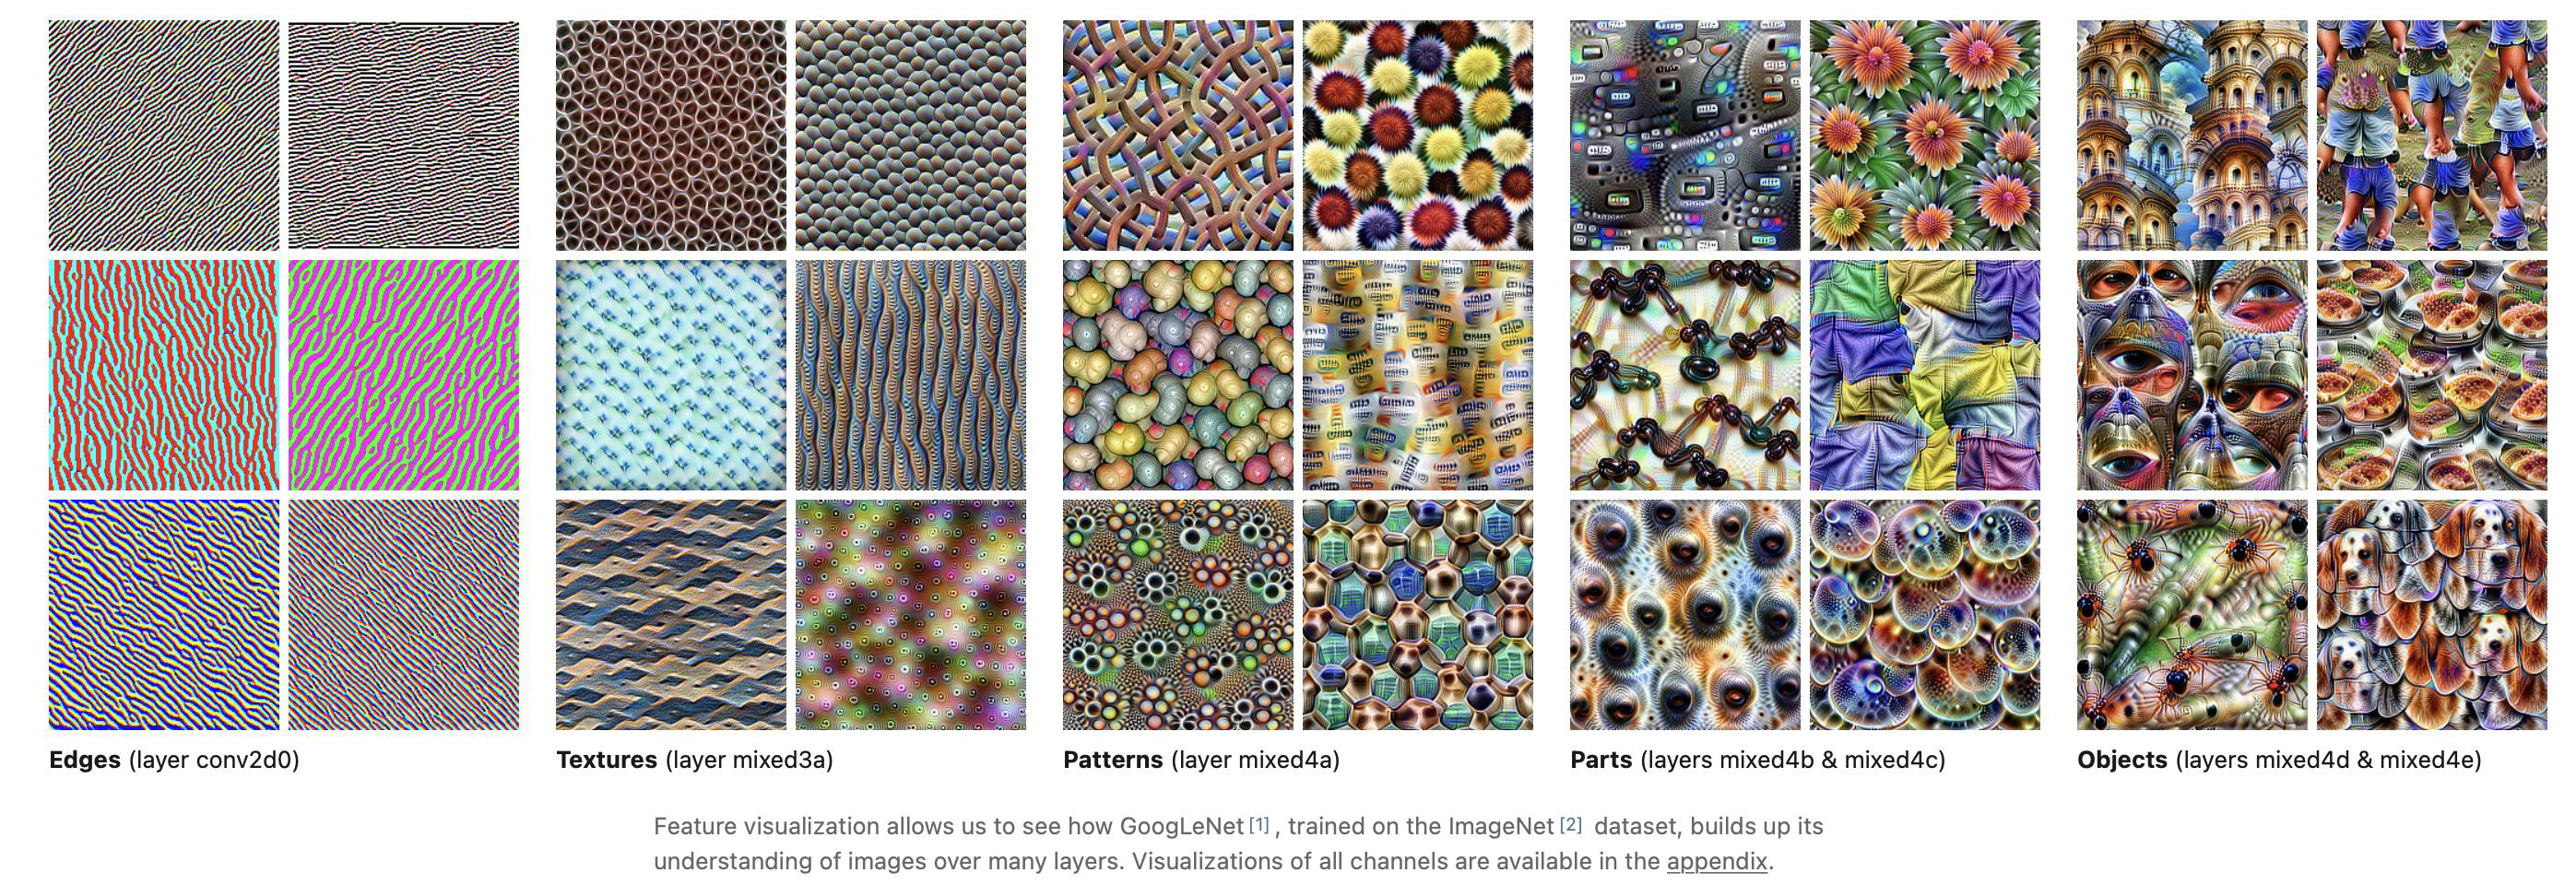
\includegraphics[width=1\linewidth]{images/week_4/visualising features 4.png}
    \caption{From textures to objects}
    \label{fig:enter-label}
\end{figure}

Feature visualization allows us to see what each neuron or layer is learning by generating images that maximize the neuron’s activation. Several types of visualizations can be used:
\begin{itemize}
    \item \textbf{Neuron visualization}: We can visualize what input maximally activates a single neuron in a particular layer (represented by $\text{layer}[x,y,z]$, where $x$ and $y$ are spatial coordinates, and $z$ is the channel index).
    \item \textbf{Channel visualization}: We can visualize the filters or kernels by optimizing for an entire feature map/channel, giving insight into what patterns that channel detects.
    \item \textbf{Layer visualization (e.g., DeepDream)}: We can perform optimization over entire layers, allowing us to understand what patterns are being captured across multiple neurons within the same layer.
    \item \textbf{Class Logits and Class Probability}: Here, we optimize for specific classes (e.g., maximizing the probability of the class “dog”), showing what features in an image are most strongly associated with that class.
\end{itemize}

\subsection*{Examples of learned features}
\begin{itemize}
    \item \textbf{Edges}: In the very first layers, CNNs learn to detect simple features such as vertical, horizontal, and diagonal edges.
    \item \textbf{Textures}: Deeper layers in the network start detecting repetitive textures. For example, a filter may learn to recognize circular textures or grids.
    \item \textbf{Patterns}: As we move deeper into the network, the filters start recognizing more complex, recurring patterns, like floral patterns or geometric structures.
    \item \textbf{Parts}: Even deeper layers can capture parts of objects (e.g., petals of a flower or fur patterns on an animal).
    \item \textbf{Objects}: In the final layers, CNNs learn full object representations by combining multiple features learned from earlier layers.
\end{itemize}

\subsection*{Why feature visualization is useful}
\begin{itemize}
    \item Feature visualization provides insight into \textbf{what the network is learning} at each layer, helping researchers and engineers understand why a CNN makes certain predictions.
    \item It helps diagnose \textbf{model weaknesses} or biases by revealing what features the network prioritizes.
    \item Feature visualization also aids in the \textbf{interpretability} of deep learning models, which is critical for applications in areas such as medicine, autonomous driving, and other safety-critical fields.
\end{itemize}
